\documentclass[stu, a4paper, 12pt, floatsintext]{apa7}

% Title Page Stuff
\title{Aerodyanamics E3 Coursework: A Report on the Supersonic Flow and Propulsion Laboratories}
\shorttitle{Aerodynamics Coursework}
\leftheader{25/03/25}
\authorsnames{Philip Beswick @00662943}
\authorsaffiliations{The University of Salford}
\course{Aerodynamics E3}
\professor{Dr Andreea Koreanschi, Dr Ali Bahr Ennil}
\duedate{25/03/25}
\abstract{This report consists of two distinct elements. Part 1 discusses the Supersonic Wind Tunnel laboratory, which aims to investigate how shockwaves form on a diamond shaped airfoil at various angles of attacks, which then compares with the known Supersonic wave theory. Part 2 discusses tests completed on the SR-30 turbojet engine located in the Aero/Mechanical Laboratory at the University of Salford. Both parts proved to be successful as each provided results that could be disucssed. Although not all results were valid, they were easily to explain and identify, using the known theory of supersonic shocks and the Brayton Cycle respectively. Ultimately, in part 1, shock waves were observed over the airfoil, which were then compared with calcualted shock angles and in part 2 the equipment was able to measure the thrust output of the SR-30, which was then comapred with a calcualted value. If further study were to be compelted, a more indepth analysis of the SR-30 would be useful in order to understand why the measured values of thrust were not as expected.}

% Packages Required
\usepackage{csquotes}
\usepackage[english]{babel}
\usepackage[T1]{fontenc}
\usepackage{mathptmx}
\usepackage{multirow}
\usepackage{graphicx}
\usepackage{booktabs}
\usepackage[style=apa,sortcites=true,sorting=nyt,backend=biber]{biblatex}
\usepackage{pgf-pie}
\usepackage{pgfplots}
\usepackage{paracol}
\usepackage{amsmath}
\usepackage{tocloft}
\usepackage{float}
\usepackage{listings}
\usepackage{gensymb}

\addbibresource{bibliography.bib}

\pgfplotsset{compat=1.18}

% Counts chapters numerically
\setcounter{tocdepth}{5}
\setcounter{secnumdepth}{5}

% Counts equations, figures and tables sequentially depending on the chapter
\numberwithin{figure}{section}
\numberwithin{table}{section}
\numberwithin{equation}{section}

\newcommand{\listequationsname}{\Large List of Equations}
\newlistof{myequations}{equ}{\listequationsname}
\newcommand{\myequations}[1]{%
\addcontentsline{equ}{myequations}{\protect\numberline{\theequation}#1}\par}
\setlength{\cftmyequationsnumwidth}{2.5em}% Width of equation number in List of Equations

% Makes sure LaTeX knows where we are :D
\DeclareLanguageMapping{british}{british-apa}

\begin{document}

\maketitle{} % Generates the title page

\tableofcontents

\newpage

\addcontentsline{toc}{subsection}{List of Figures}
\listoffigures
\addcontentsline{toc}{subsection}{List of Tables}
\listoftables
\addcontentsline{toc}{subsection}{List of Equations}
\listofmyequations

%%% Contents of report go here %%%
\newpage
\section{Supersonic Flow Laboratory}
\subsection{Aims and Objectives}
The procedure aims to use a Schlieren system to observe the shockwave structures on a diamond aerofoil when orientated at different angles of attack but in a constant air flow of Mach 1.8. Objectives of this procedure include obtaining numerical and physical results that can be compared with theory and gaining technical skills, such as familiarity with the equipment used.
\subsection{Description of Theoretical Expectations}
As the diamond airfoil has been placed in a flow regime where the freestream Mach number is 1.8, shock waves will be expected to form. These shocks will form about the leading edge point, trailing edge point and expansion fans at the shoulders of the diamond airfoil. Furthermore, in \textit{Aerodynamics}, Clancy suggests that with an increasing angle of attack, the shocks may become detached from the leading edge(\cite{Clancy1986}). To keep the shocks attached to the leading edge, the free stream Mach number would have to increase; in this procedure, this remains constant. When the angle of attack further increases, a bow, detached shock is expected to occur ahead of the leading edge(\cite{Clancy1986}). 
\subsection{Description of Experimental Procedure}
Before the testing of the diamond airfoil at different angles of attacks can take place, the supersonic wind tunnel must be prepared. Preparation involves:
\begin{itemize}
    \item Fitting the appropriate liner to the tunnel to achieve the desired free stream Mach number (in this case, a liner to achieve Mach 1.8 was attached).
    \item The model must be secured in the tunnel’s testing section.
    \item The Schlieren apparatus must be set up.
\end{itemize}
Once this has been completed, the angle of attack of the model must be set by the tunnel operators, and then the tunnel bypass valve can be opened. Then, the tunnel vacuum pump can be starte,d and once it reaches full speed, the bypass valve should again be shut. At this stage, pressure and Mach numbers were recorded for the tunnel at 25 different pressure tapping points. This data is then saved to a spreadsheet for post-processing. Concurrently, the Schlieren apparatus will be displaying the model and (if present) any shocks that are occurring. Once all data has been collected, the bypass valve is opened, the tunnel is stopped and these steps previously outlined are repeated for the following angles of attacks: 0 degrees, 2 degrees, 4 degrees, 6 degrees and 8 degrees. 
\subsection{Description of Experimental Outcomes}
Upon completion of the procedure, Schlieren images for each angle of attack were recorded. These can be found in Figures 1.1 to 1.5.
\begin{figure}[H]
    \caption{The Schlieren Image Produced at an Angle of Attack of 0$\degree$.}
    \label{fig:aero_zero}
    \centering
    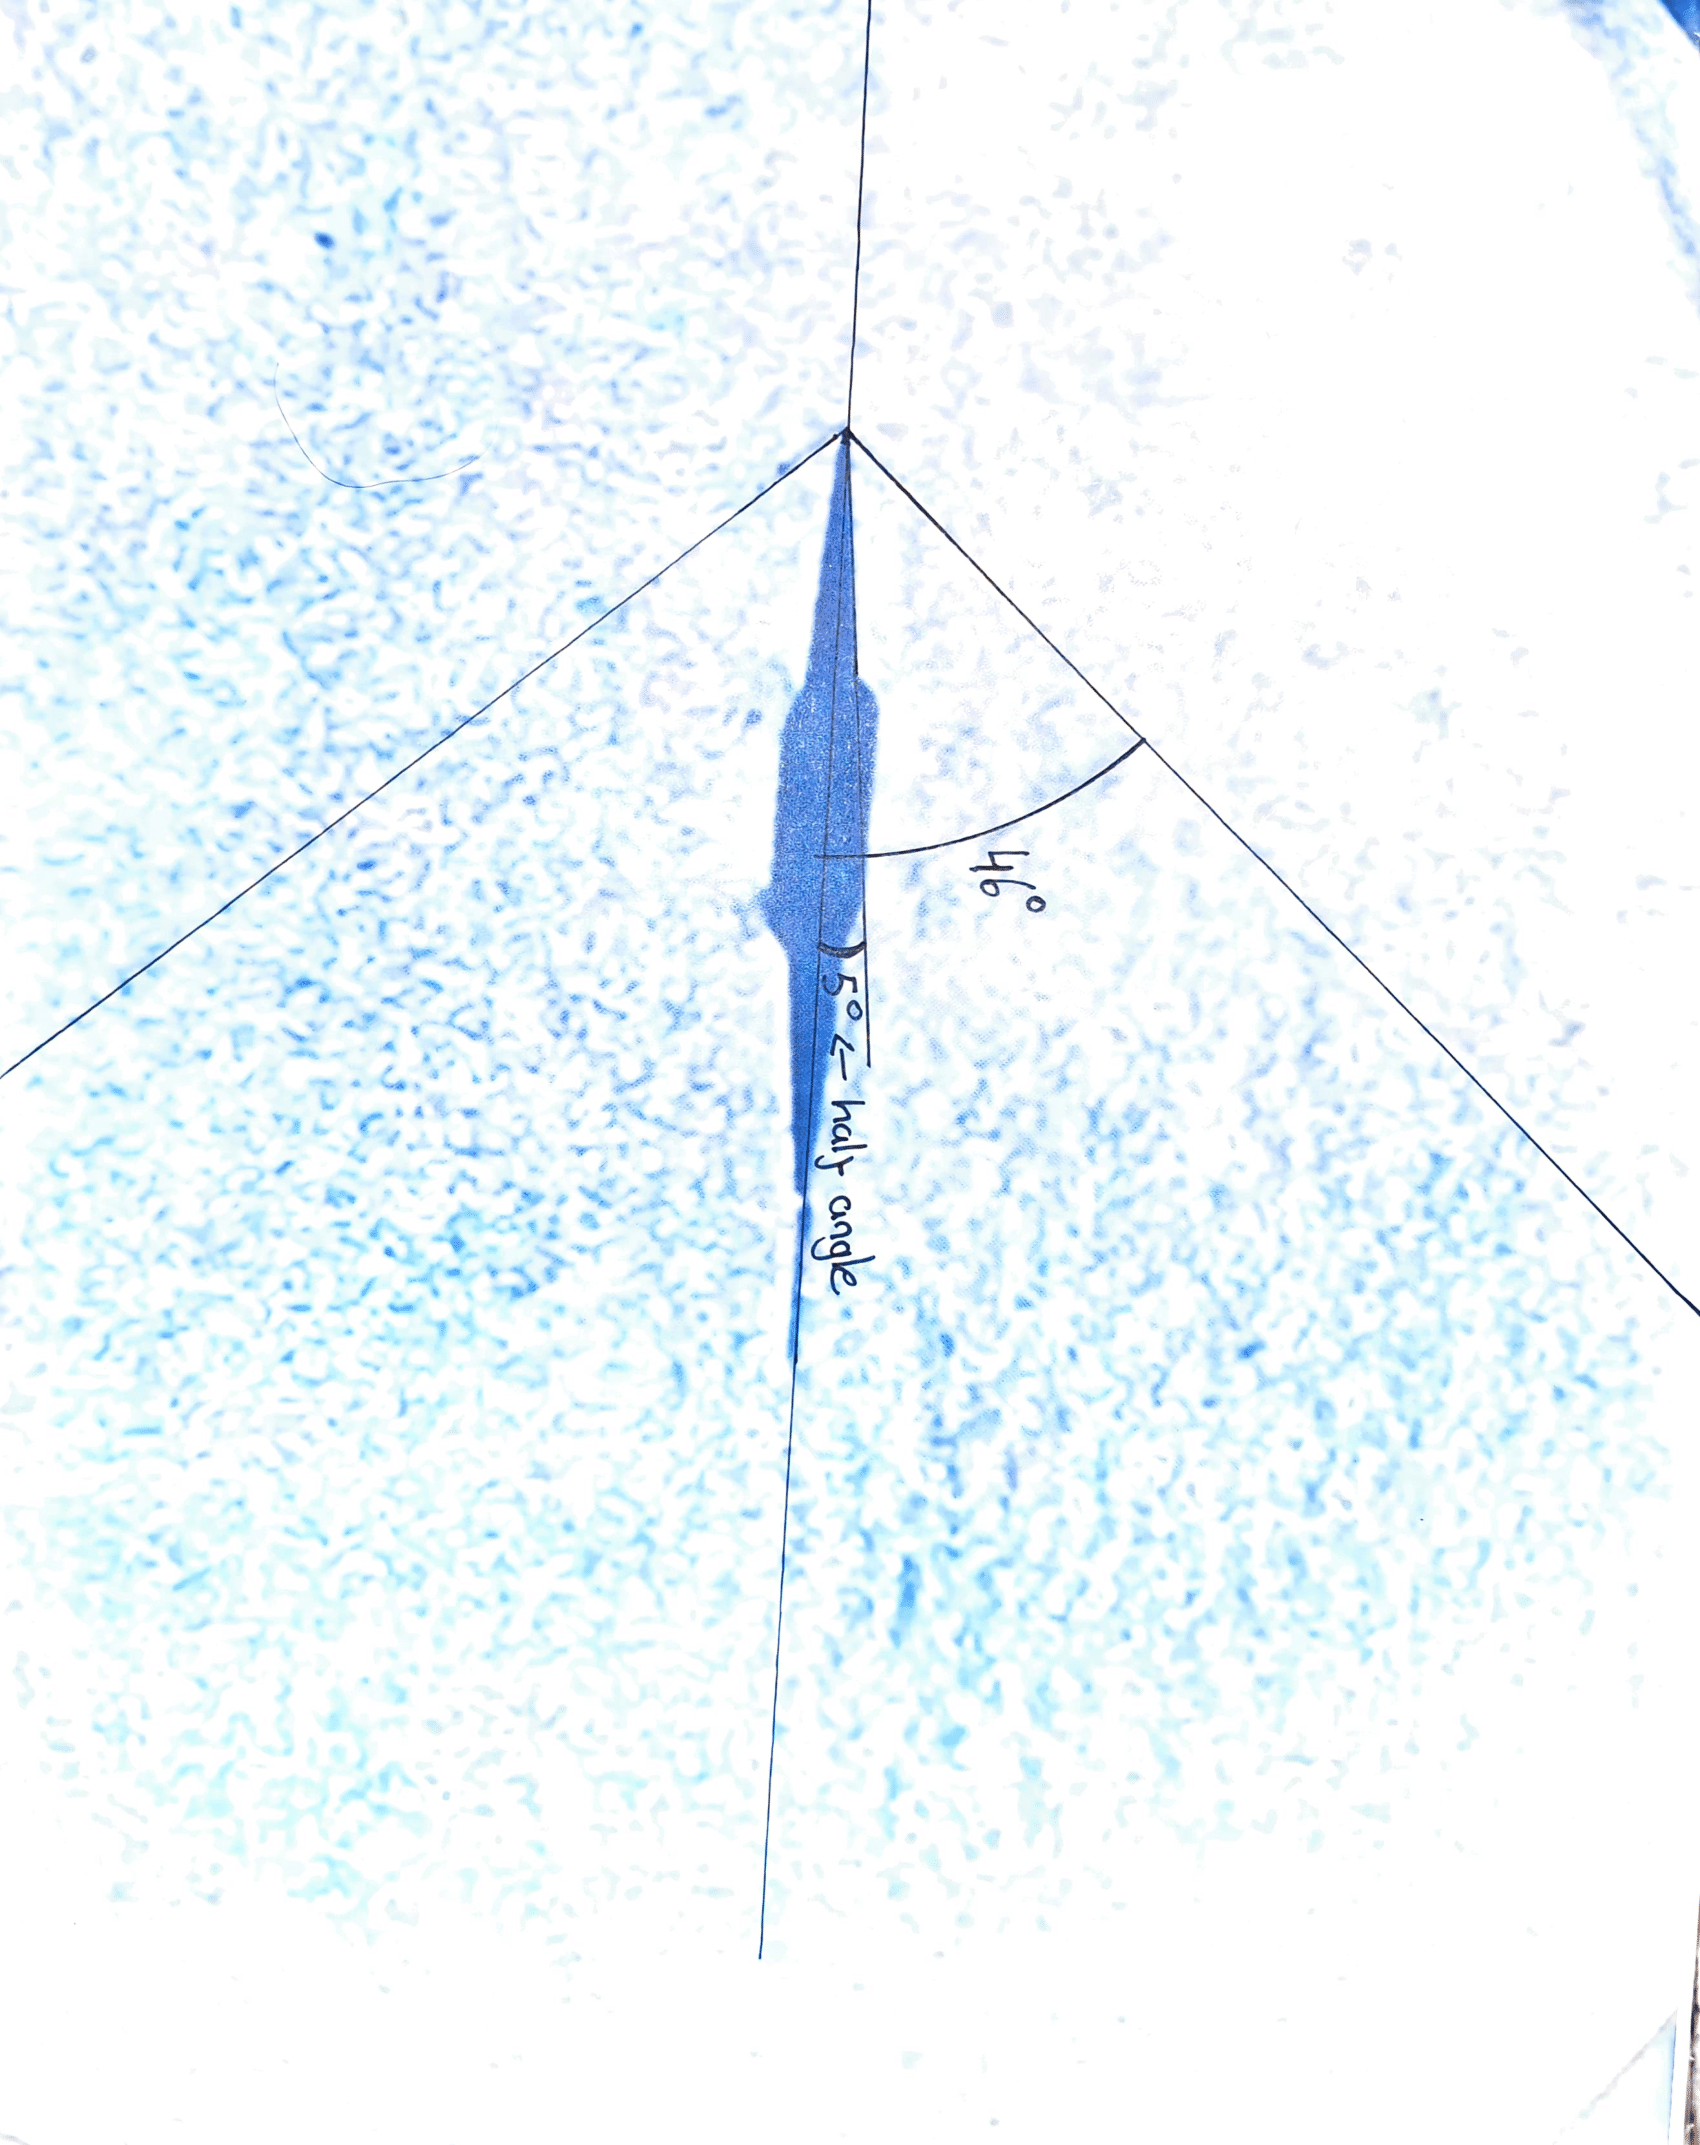
\includegraphics[width=1.0\textwidth]{pictures/zero.png}
\end{figure}
\begin{figure}[H]
    \caption{The Schlieren Image Produced at an Angle of Attack of 2$\degree$.}
    \label{fig:aero_two}
    \centering
    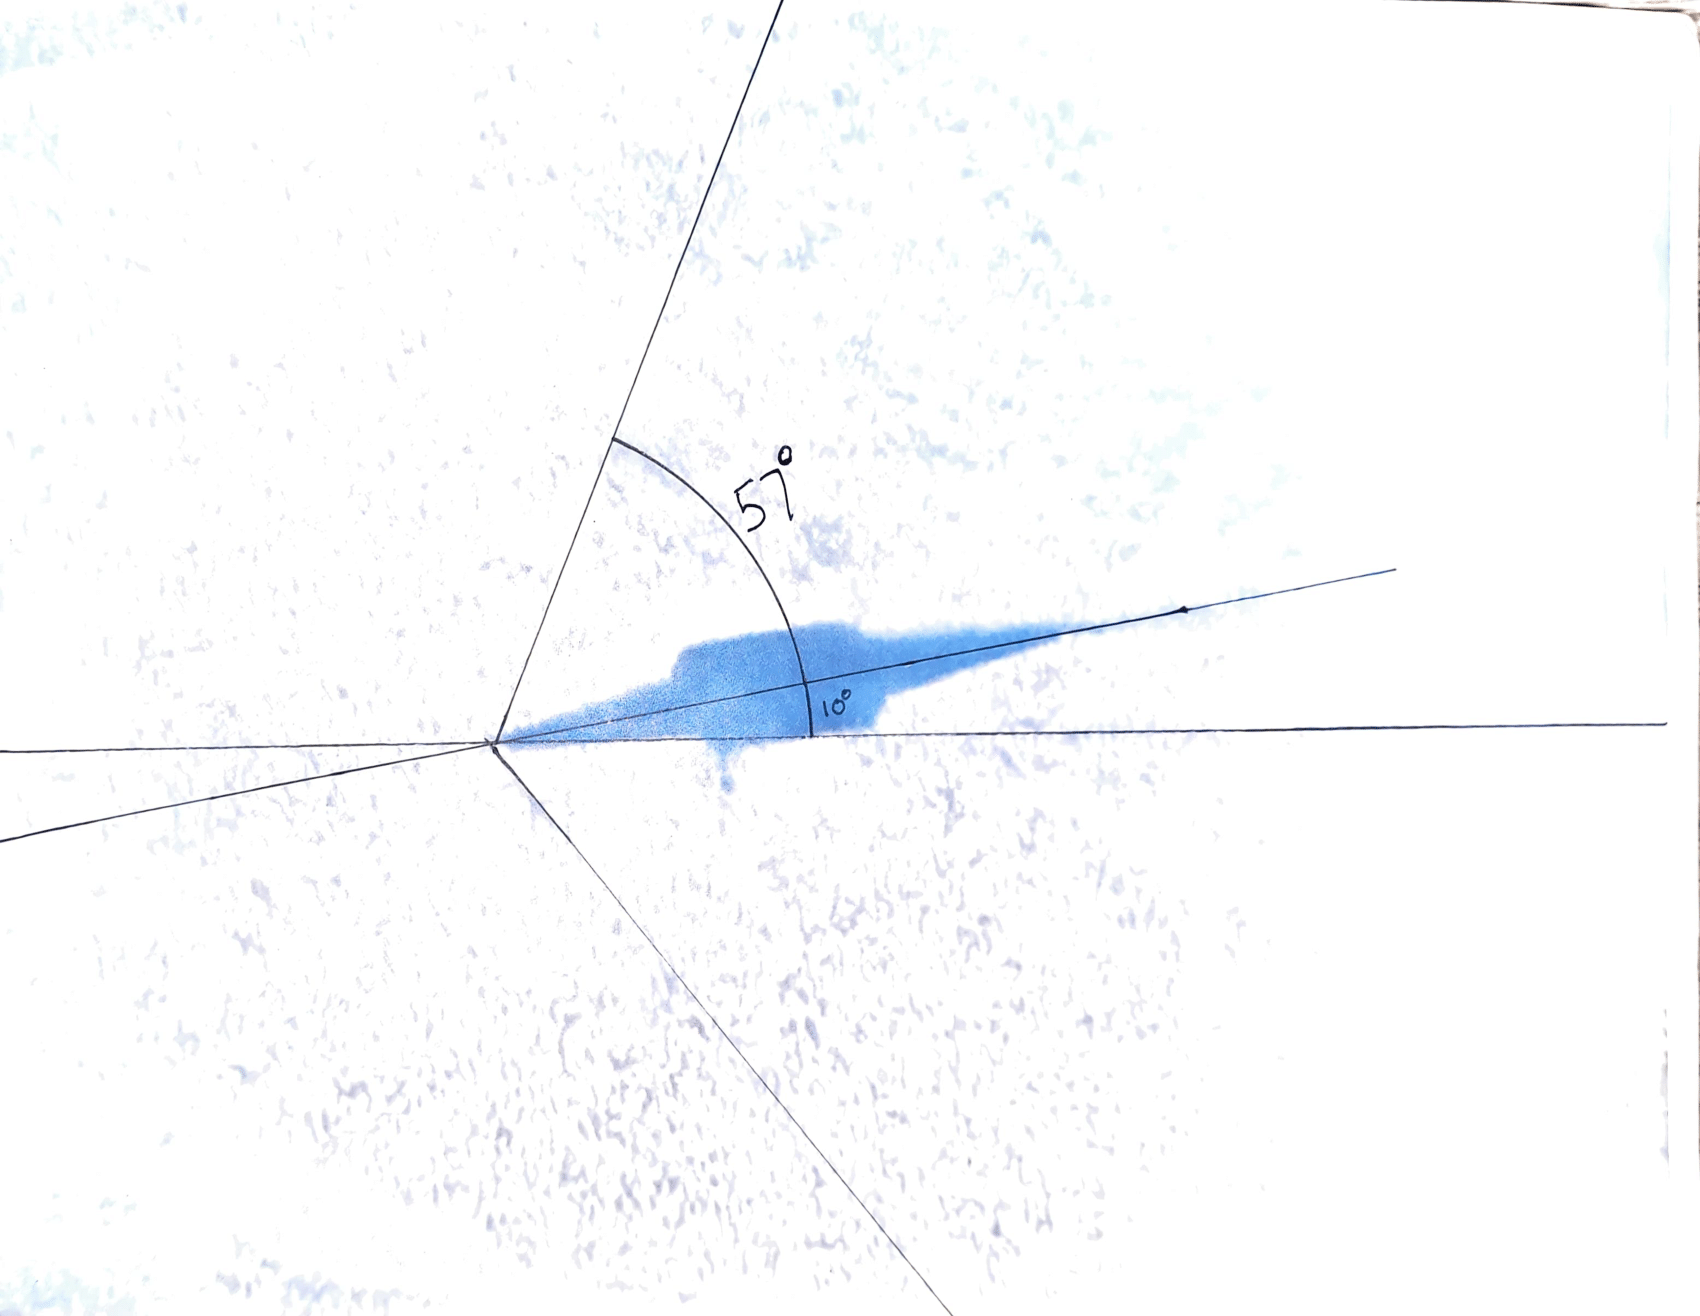
\includegraphics[width=1.0\textwidth]{pictures/two.png}
\end{figure}
\begin{figure}[H]
    \caption{The Schlieren Image Produced at an Angle of Attack of 4$\degree$.}
    \label{fig:aero_four}
    \centering
    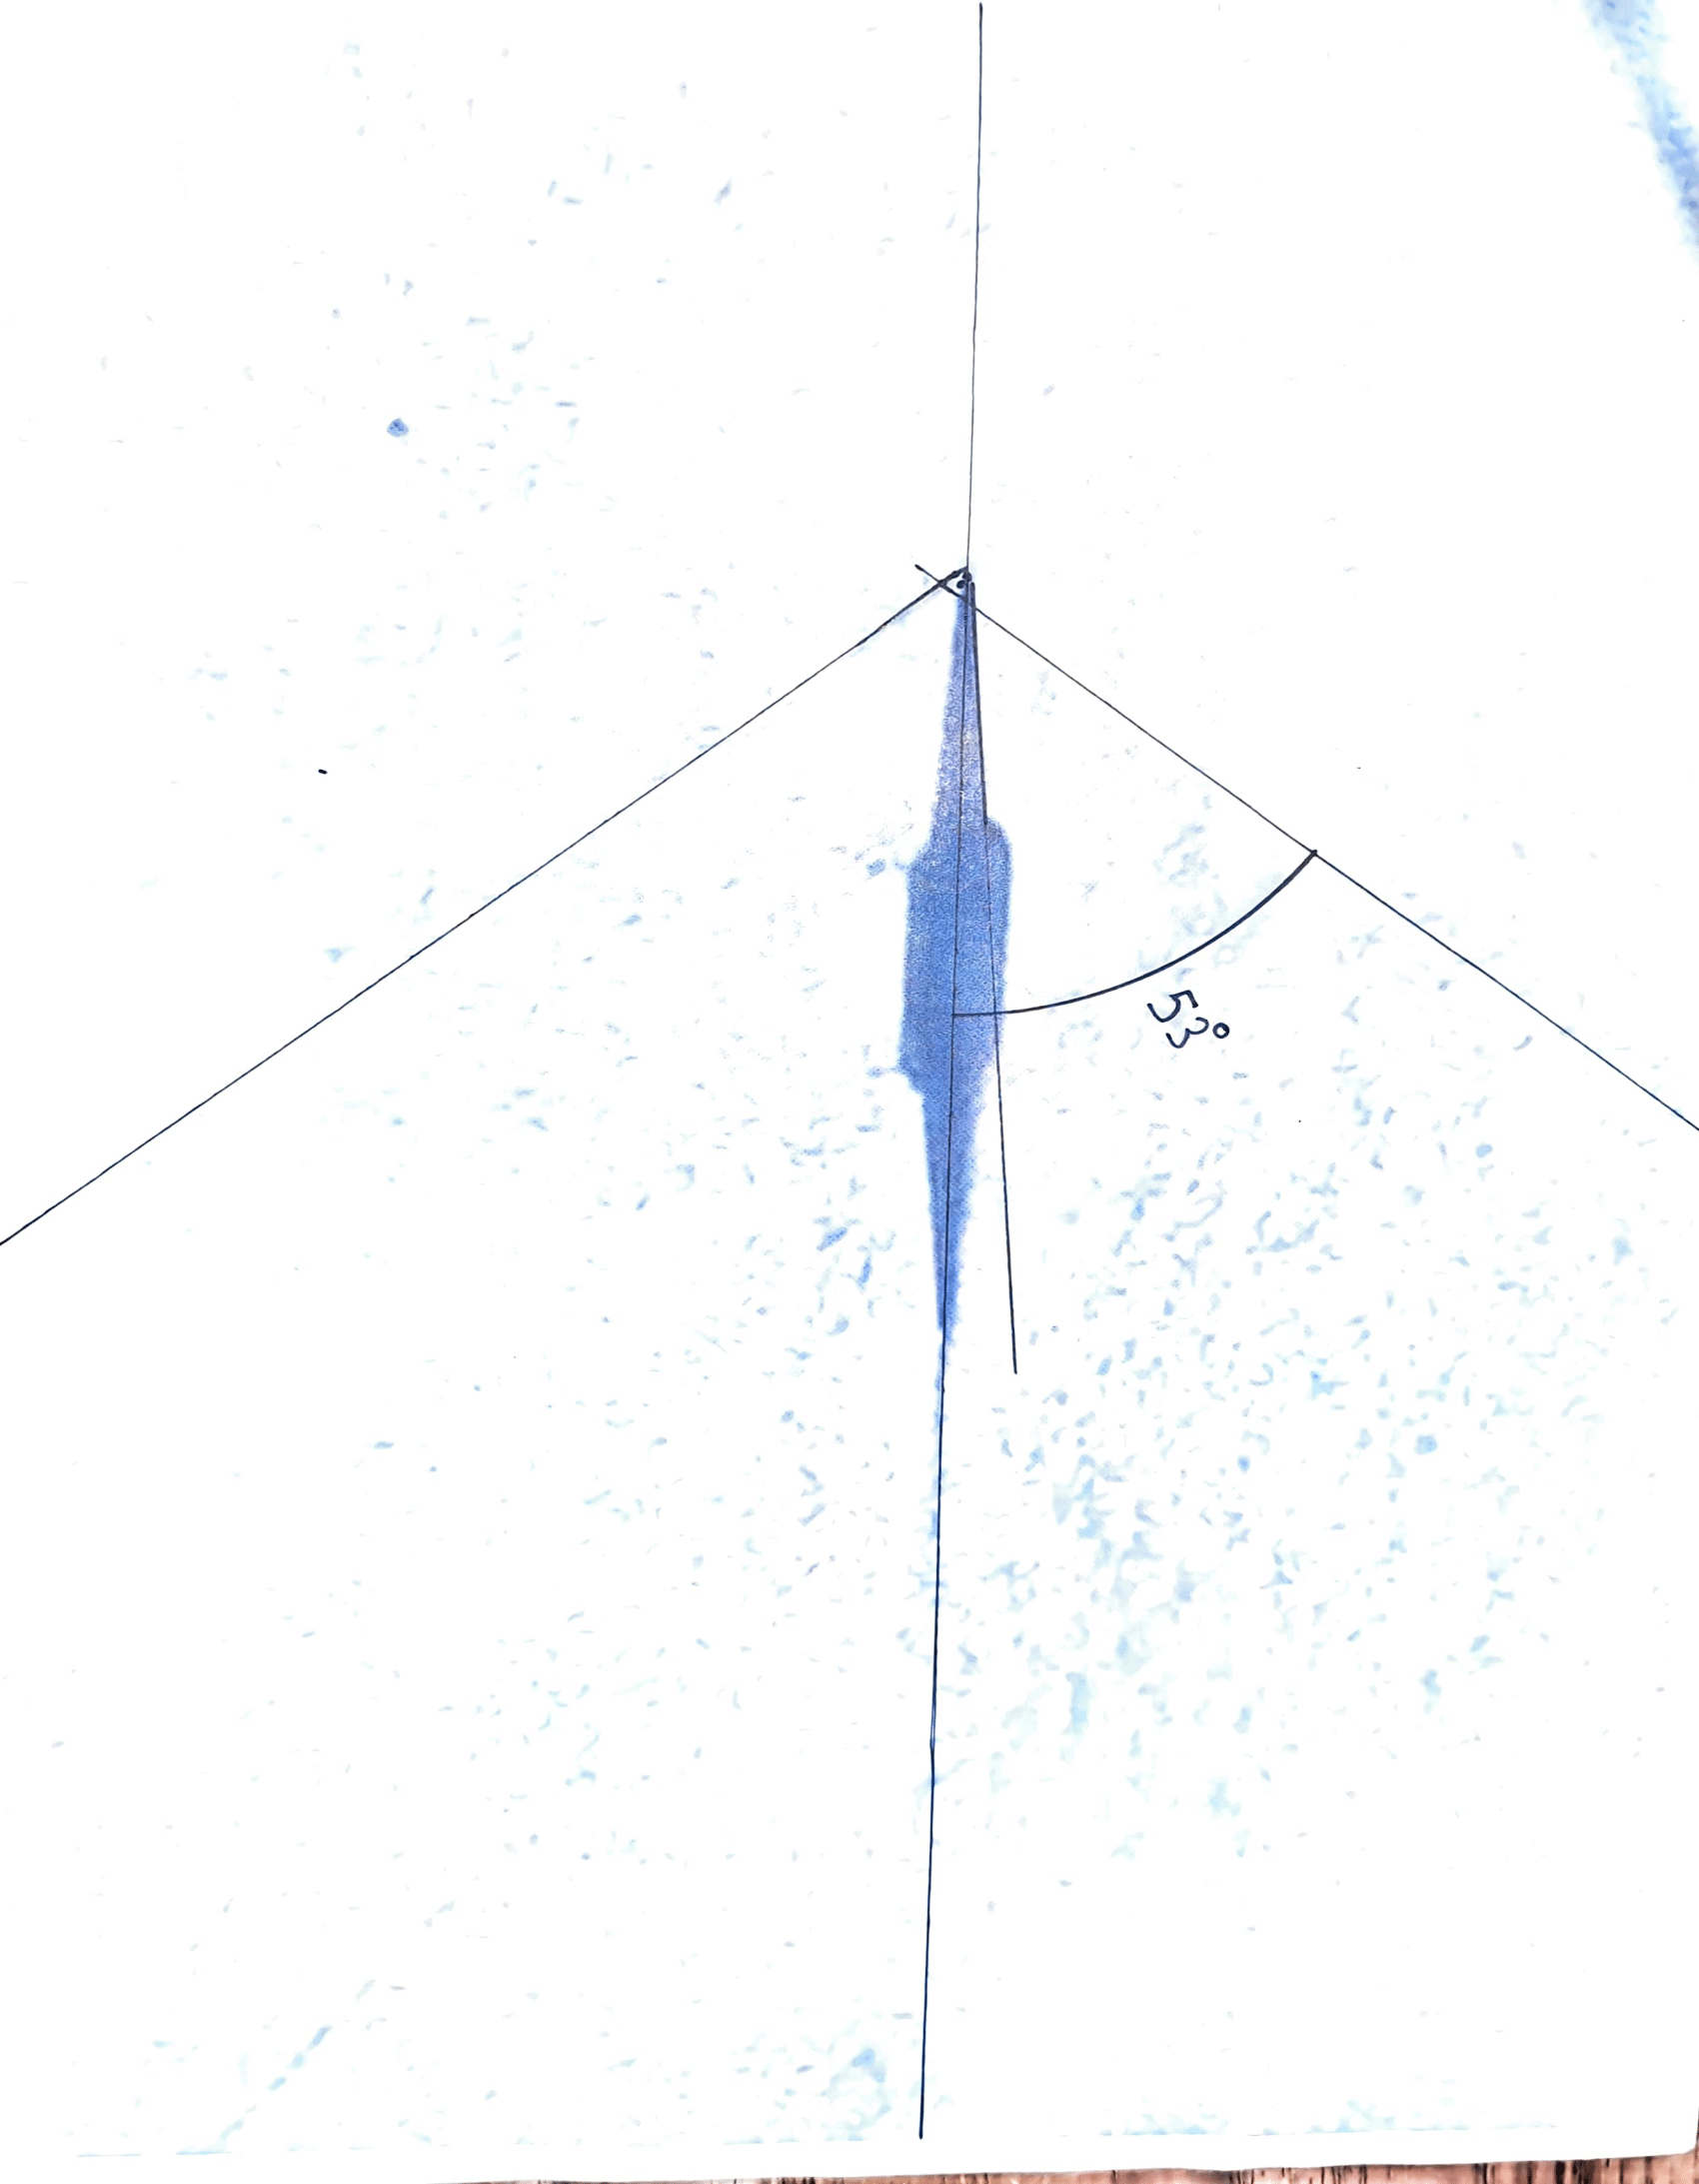
\includegraphics[width=1.0\textwidth]{pictures/four.png}
\end{figure}
\begin{figure}[H]
    \caption{The Schlieren Image Produced at an Angle of Attack of 6$\degree$.}
    \label{fig:aero_six}
    \centering
    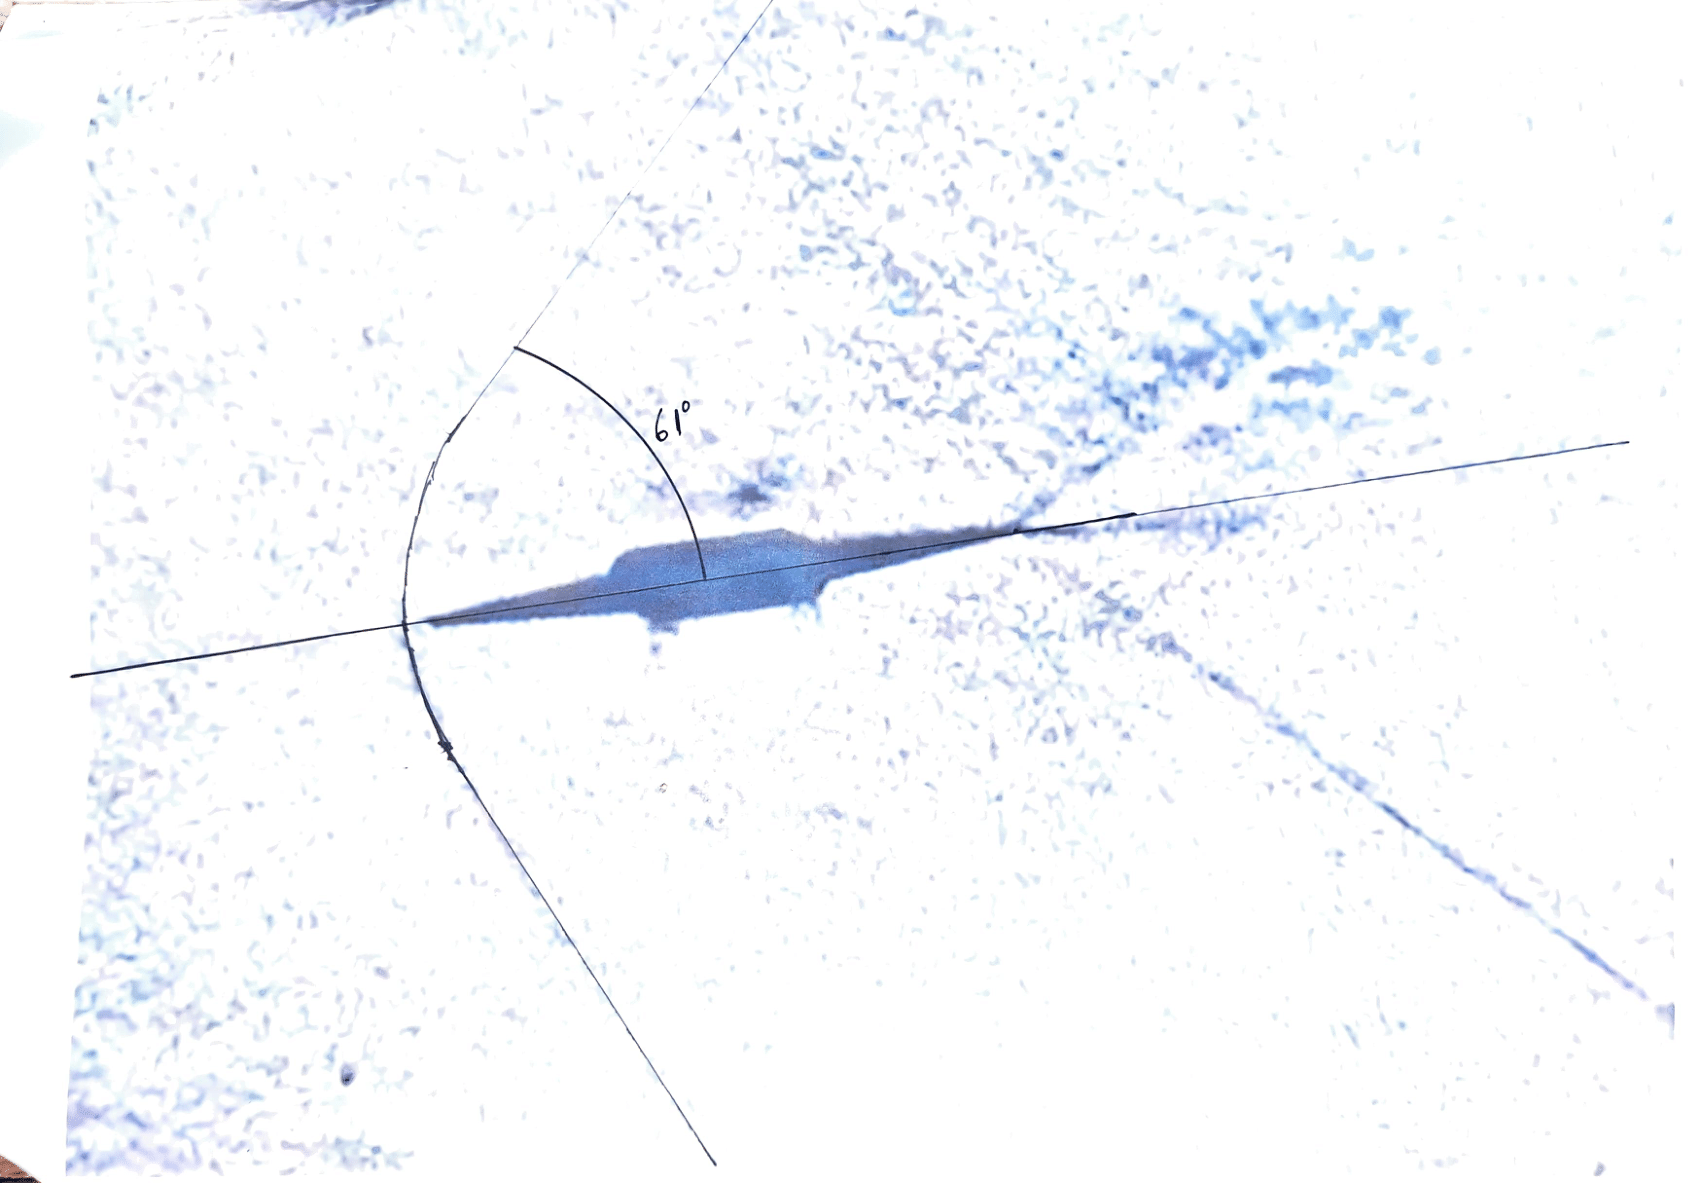
\includegraphics[width=1.0\textwidth]{pictures/six.png}
\end{figure}
\begin{figure}[H]
    \caption{The Schlieren Image Produced at an Angle of Attack of 8$\degree$.}
    \label{fig:aero_eight}
    \centering
    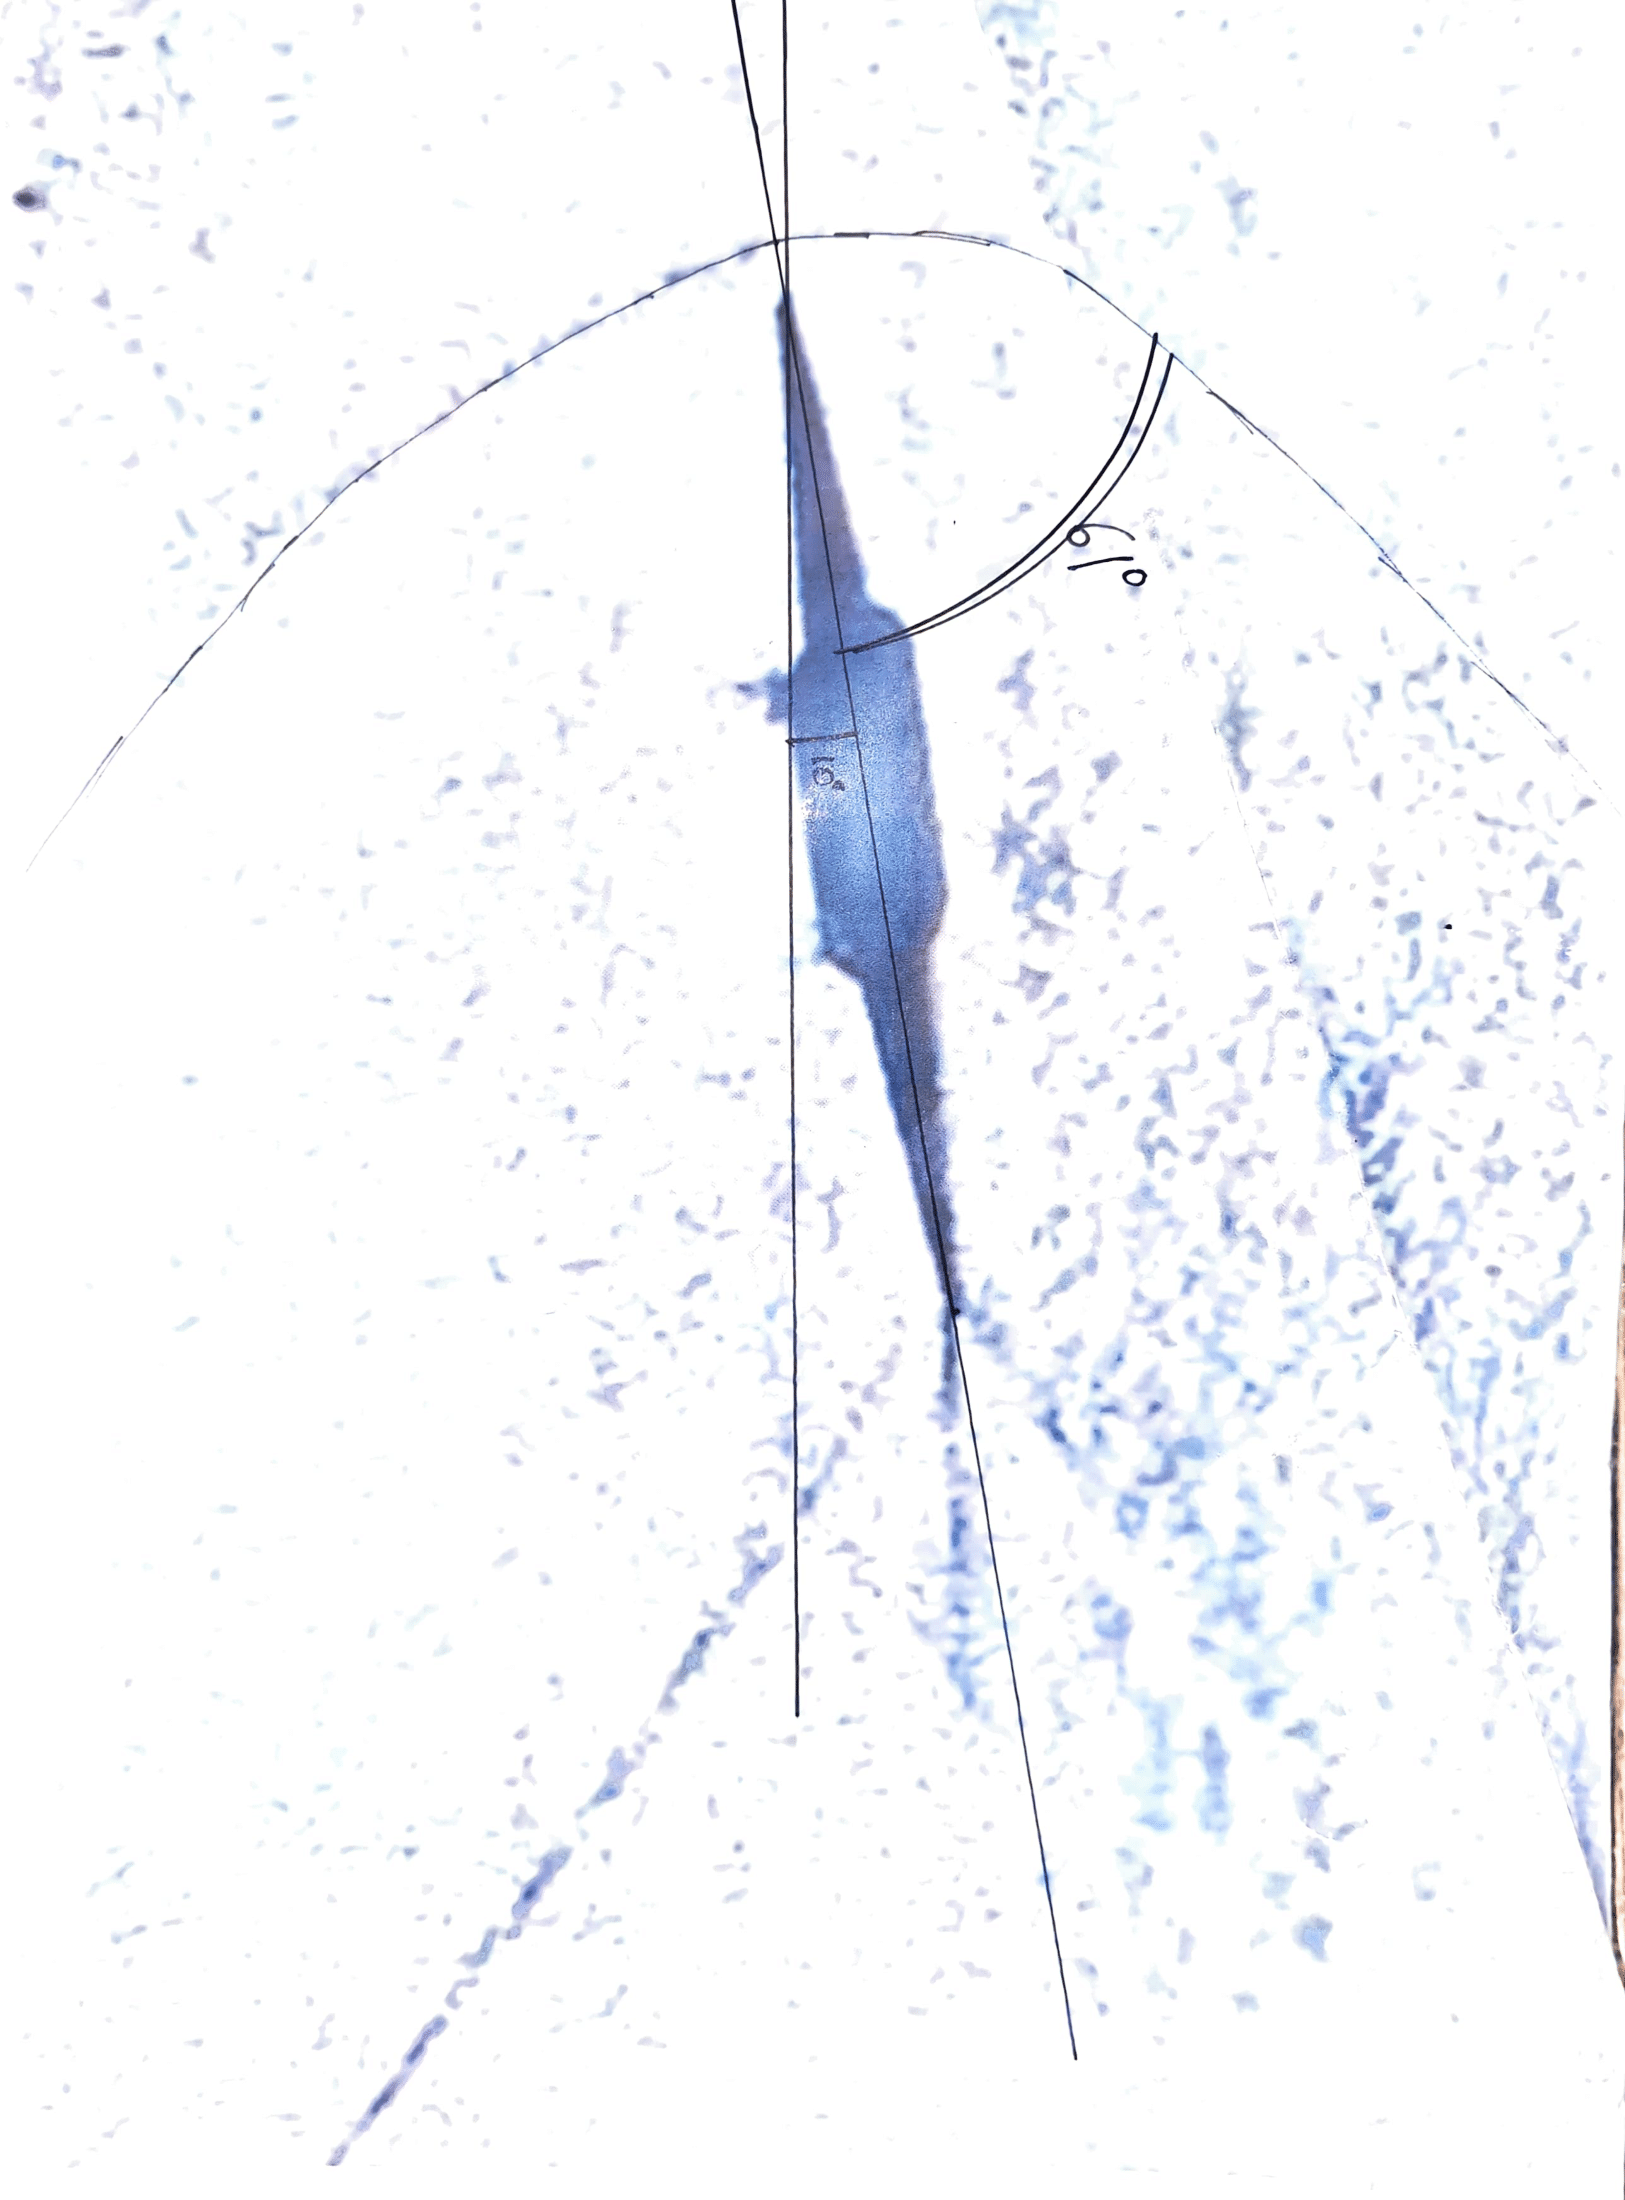
\includegraphics[width=1.0\textwidth]{pictures/eight.png}
\end{figure}
These figurs show that as angle of attack increases, the shock angle also increases, although there are anomalous results for angles of 2$\degree$ and 4$\degree$. 
In addition to the Schlieren images produced, values of local pressure were taken at 25 unique points in the tunnel's testing section. These results can be found in Table 1.1.
\begin{table}[H]
    \centering
    \caption{Values of pressure with varying angle of attack at each pressure tapping point.}
    \label{tab:local_pressure_table}
    \resizebox{\columnwidth}{!}{%
        \begin{tabular}{@{}cccccccccccccccccccccccccc@{}}
            \toprule
            \textbf{Model   Angle} & \multicolumn{25}{c}{\textbf{Corrected Pressures (Pa)}}                                                                                                                                                \\ \midrule
            (degrees)              & 1     & 2     & 3     & 4     & 5     & 6     & 7     & 8     & 9     & 10    & 11    & 12    & 13    & 14    & 15    & 16    & 17    & 18    & 19    & 20    & 21    & 22    & 23    & 24    & 25    \\
            0                      & 89800 & 83900 & 82500 & 78200 & 72100 & 65000 & 57300 & 48100 & 48360 & 32900 & 24980 & 22700 & 22450 & 22240 & 21360 & 20770 & 20600 & 19890 & 18400 & 18980 & 27690 & 18300 & 22260 & 30920 & 35330 \\
            2                      & 89800 & 83900 & 82500 & 78200 & 72100 & 65000 & 57300 & 48100 & 48060 & 32740 & 24900 & 22700 & 23070 & 22300 & 21300 & 20700 & 20600 & 19900 & 18400 & 23020 & 27090 & 18500 & 21980 & 30680 & 35050 \\
            4.1                    & 89800 & 83900 & 82500 & 78200 & 72100 & 65000 & 57300 & 48100 & 48230 & 32790 & 24900 & 22700 & 22890 & 22280 & 21330 & 20700 & 20600 & 19900 & 18410 & 28800 & 26290 & 19150 & 26830 & 33310 & 36340 \\
            5.9                    & 89800 & 83900 & 82500 & 78200 & 72100 & 65000 & 57300 & 48100 & 48330 & 32850 & 24930 & 22700 & 22880 & 22310 & 21360 & 20700 & 20600 & 19900 & 18840 & 31250 & 26080 & 22290 & 30130 & 34850 & 37260 \\
            7.9                    & 89800 & 83900 & 82500 & 78200 & 72100 & 65000 & 57300 & 48100 & 48430 & 32930 & 24970 & 22690 & 22740 & 22300 & 21380 & 20710 & 20600 & 19900 & 29670 & 30230 & 29770 & 34460 & 37250 & 39510 & 40970 \\ \bottomrule
        \end{tabular}%
    }
\end{table}
The pressure distribution for each of the angles of attack measured can be found below in Figure 1.6. 
\begin{figure}[H]
    \caption{Pressure Distribution for various Angles of Attack}
    \label{fig:aero_pressures}
    \centering
    \resizebox{1\textwidth}{!}{%
    \begin{tikzpicture}
        \begin{axis}[
            title={},
            xlabel={Tapping Position on X Axis},
            ylabel={Pressure Corrected for Tunnel Conditions [Pa]},
            xmin=0, xmax=700,
            ymin=0, ymax=100000,
            xtick={0,100, 200, 300, 400, 500, 600, 700},
            ytick={0,10000, 20000, 30000, 40000, 50000, 60000, 70000, 80000, 90000, 100000},
            legend pos=north east,
            ymajorgrids=true,
            grid style=dashed,
        ]
        
        \addplot[
            color=blue,
            mark=square,
            ]
            coordinates {
                (19.5, 89800)	(44.5, 83900)	(69.5, 82500)	(94.5, 78200)	(119.5, 72100)	(144.5, 65000)	(169.5, 57300)	(194.5, 48100)	(194.5, 48360)	(219.5, 32900)	(244.5, 24980)	(269.5, 22700)	(294.5, 22450)	(319.5, 22240)	(344.5, 21360)	(369.5, 20770)	(394.5, 20600)	(419.5, 19890)	(444.5, 18400)	(469.5, 18980)	(519.5, 27690)	(544.5, 18300)	(569.5, 22260)	(594.5, 30920)	(619.5, 35330)
            };
        \addplot[
            color=red,
            mark=triangle,
            ]
            coordinates {
                (19.5, 89800)	(44.5, 83900)	(69.5, 82500)	(94.5, 78200)	(119.5, 72100)	(144.5, 65000)	(169.5, 57300)	(194.5, 48100)	(194.5, 48060)	(219.5, 32740)	(244.5, 24900)	(269.5, 22700)	(294.5, 23070)	(319.5, 22300)	(344.5, 21300)	(369.5, 20700)	(394.5, 20600)	(419.5, 19900)	(444.5, 18400)	(469.5, 23020)	(519.5, 27090)	(544.5, 18500)	(569.5, 21980)	(594.5, 30680)	(619.5, 35050)
            };
        \addplot[
            color=green,
            mark=circle,
            ]
            coordinates {
                (19.5, 89800)	(44.5, 83900)	(69.5, 82500)	(94.5, 78200)	(119.5, 72100)	(144.5, 65000)	(169.5, 57300)	(194.5, 48100)	(194.5, 48230)	(219.5, 32790)	(244.5, 24900)	(269.5, 22700)	(294.5, 22890)	(319.5, 22280)	(344.5, 21330)	(369.5, 20700)	(394.5, 20600)	(419.5, 19900)	(444.5, 18410)	(469.5, 28800)	(519.5, 26290)	(544.5, 19150)	(569.5, 26830)	(594.5, 33310)	(619.5, 36340)
            };
        \addplot[
            color=yellow,
            mark=pentagon,
            ]
            coordinates {
                (19.5, 89800)	(44.5, 83900)	(69.5, 82500)	(94.5, 78200)	(119.5, 72100)	(144.5, 65000)	(169.5, 57300)	(194.5, 48100)	(194.5, 48330)	(219.5, 32850)	(244.5, 24930)	(269.5, 22700)	(294.5, 22880)	(319.5, 22310)	(344.5, 21360)	(369.5, 20700)	(394.5, 20600)	(419.5, 19900)	(444.5, 18840)	(469.5, 31250)	(519.5, 26080)	(544.5, 22290)	(569.5, 30130)	(594.5, 34850)	(619.5, 37260)
            };
        \addplot[
            color=purple,
            mark=hexagon,
            ]
            coordinates {
                (19.5, 89800)	(44.5, 83900)	(69.5, 82500)	(94.5, 78200)	(119.5, 72100)	(144.5, 65000)	(169.5, 57300)	(194.5, 48100)	(194.5, 48430)	(219.5, 32930)	(244.5, 24970)	(269.5, 22690)	(294.5, 22740)	(319.5, 22300)	(344.5, 21380)	(369.5, 20710)	(394.5, 20600)	(419.5, 19900)	(444.5, 29670)	(469.5, 30230)	(519.5, 29770)	(544.5, 34460)	(569.5, 37250)	(594.5, 39510)	(619.5, 40970)
            };
            \legend{0$\degree$, 2$\degree$, 4$\degree$, 6$\degree$, 8$\degree$}
        \end{axis}
    \end{tikzpicture}
    }
\end{figure}
It is important to note that Figure 1.6 has the values of pressure that have been corrected accounting for atmospheric pressure and are therefore true, values of pressure for each pressure tapping location. The model is also tested upside down in the tunnel, hence the shape of the graph roughly appearing to be the mirror image of what is expected.
\subsection{Discussion}
Overall, the Schlieren images seen in Figures 1.1 to 1.5 do tend to match the theory suggested by Clancy in \textit{Aerodynamics} (\cite{Clancy1986}). As the angle of attack increases, the shocks both detach from the leading edge and become more similar to a bow shock, rather than a normal one. The only difference is that expansion fans are not present in the Schlieren images. This is likely due to the small area of the testing section, which will prevent their development due to boundary layer conditions interfering with the flow around the diamond airfoil. 
\begin{table}[H]
    \centering
    \caption{Calculated values of shock angles}
    \label{tab:aero_shock_angles}
    \begin{tabular}{@{}ccc@{}}
    \toprule
    \textbf{Model   Angle} & \textbf{Free Steam Mach Number} & \textbf{Shock Angle} \\ \midrule
    (degrees)              & (Mach)                          & (degrees)            \\
    0                      & 1.8                             & 38.44                \\
    2                      & 1.8                             & 40.56                \\
    4.1                    & 1.8                             & 42.96                \\
    5.9                    & 1.8                             & 45.2                 \\
    7.9                    & 1.8                             & 47.97                \\ \bottomrule
    \end{tabular}
\end{table}
Also, the values of the calculated shock angle, seen in Table 1.2 are very different from the values measured in Figures 1.1 to 1.5. Again, the impact of the wind tunnel walls may result in different shock angles when measuring and calculating. The calculated values assume absolutely ideal conditions (steady, inviscid and adiabatic flow with no body forces), ultimately these are not realistic conditions when operating in a wind tunnel. In addition, the angles on the Schlieren images were measured by first taking a picture of the image displayed on a monitor, and then physically measuring with a protractor. Here, a great deal of inaccuracy has occurred, which will result in shock angles that are not absolutely correct. Therefore, it is likely that both methods have inaccuracies (although different in nature) and is therefore unsurprising why they therefore give different results.
The shock angles were calculated using the relation between the flow angle, $\theta$, the shock angle $\beta$ and the flow freestream velocity, $M$ which takes the value of 1.8.
\begin{equation}
    tan(\theta) = 2cot(\beta) {{M^2sin^2(\beta)-1}\over{M^2(\gamma+cos(2\beta)+2)}} \, ,
\end{equation}
\myequations{Equation to find shock angles.}
The methodology for how this equation was applied will be discussed in the Appendix. 

\newpage
\section{Propulsion Laboratory}
\subsection{Aims and Objectives}
The experimental procedure conducted aims to produce data which can be used to analyse the performance of a small turbojet engine, while this report will discuss said data and suggest how effective the procedure was as a whole. The objectives of this laboratory are twofold: 
\begin{enumerate}
    \item To examine the performance of a small-scale turbojet engine operating at speeds up to 70000 rpm. 
    \item To gain a good understanding of the thermodynamic performance of a gas turbine engine operating on the Brayton cycle. 
\end{enumerate}
\subsection{Equipment Description}
The turbojet engine used in this procedure was the SR-30, which was mounted to the TTL Mini-Lab test bench. This engine has a centrifugal flow compressor, a reverse flow annular combustor and an axial flow turbine. Furthermore, it’s powered by kerosene fuel. In addition, the engine is equipped with four thermocouple temperature sensors and four pressure sensors, which makes the analysis of the engine’s performance possible. All data is collected by a connected computer, which monitors all of the previously mentioned sensors as well as fuel flow, thrust and RPM. The TTL Mini-Lab test bench controls the starting procedure of the engine as well as a lever, which controls the power (changes RPM) of the engine. 
\subsection{Experimental Methodology}
Due to the potentially hazardous nature of this procedure, several precautions were taken to ensure the lab operated safely. These were:
\begin{itemize}
    \item Ear protection (to EN352-2 standards) was worn at all times (\cite{BSI_HearingProtectors}). 
    \item No naked flames were used due to the flammable nature of the kerosene fuel.
    \item Safety covers were in place due to the high running speeds of the engine.
    \item The exhaust system was not approached due to the high temperature the engine runs at.
    \item The room was well ventilated due to the high oxygen use of the engine. All exhaust gasses were dispersed outside of the building. 
\end{itemize}
As all health and safety precautions were undertaken, the operation of the SR-30 could proceed. A laboratory technician started the engine to achieve a steady, idle RPM. Once this has been achieved, the power handle on the TTL Mini-Lab bench is set to give an engine RPM of 50000. Once the engine is performing steadily at this speed, the computer is set to record data for 1 minute, the computer takes several readings during this time. This is repeated for speeds of 60000 RPM and 70000 RPM until the engine is set back to idle and then shut down.
\subsection{Experimental Observations}
As the procedure was conducted, the most notable observation is that the SR-30 got increasingly louder as the RPM was increased. Furthermore, the increased speed of the engine was visible in the behaviour of the flame in the combustor, which became increasingly stretched as the RPM increased.
\subsection{Experimental Data}
\begin{figure}[H]
    \caption{This graph shows the relationship between the RPM of the SR-30 and it's Isentropic Efficiency}
    \label{fig:propulsion_rpmVSiseEff}
    \centering
    \resizebox{1\textwidth}{!}{%
    \begin{tikzpicture}
        \begin{axis}[
            title={},
            xlabel={Turbojet Shaft Speed (RPM)},
            ylabel={Isentropic Efficiency},
            xmin=0, xmax=80000,
            ymin=64.0, ymax=74.0,
            xtick={0,10000, 20000, 30000, 40000, 50000, 60000, 70000, 80000},
            ytick={64.0, 65.0, 66.0, 67.0, 68.0, 69.0, 70.0, 71.0, 72.0, 73.0, 74.0},
            ymajorgrids=true,
            grid style=dashed,
        ]
        
        \addplot[
            color=blue,
            mark=square,
            ]
            coordinates {
                (50195, 73.2)	(60413, 65.8)	(70073, 64.6)
            };
        \end{axis}
    \end{tikzpicture}
    }
\end{figure}

\begin{figure}[H]
    \caption{This graph shows the relationship between the Pressure Ratio of the SR-30 and it's Isentropic Efficiency}
    \label{fig:propulsion_pressureVSiseEff}
    \centering
    \resizebox{1\textwidth}{!}{%
    \begin{tikzpicture}
        \begin{axis}[
            title={},
            xlabel={Pressure Ratio [P1/P2]},
            ylabel={Isentropic Efficiency},
            xmin=0, xmax=2.50,
            ymin=64.0, ymax=74.0,
            xtick={0.00, 0.50, 1.00, 1.50, 2.00, 2.50},
            ytick={64.0, 65.0, 66.0, 67.0, 68.0, 69.0, 70.0, 71.0, 72.0, 73.0, 74.0},
            ymajorgrids=true,
            grid style=dashed,
        ]
        
        \addplot[
            color=blue,
            mark=square,
            ]
            coordinates {
                (1.58, 73.2)	(1.91, 65.8)	(2.34, 64.6)
            };
        \end{axis}
    \end{tikzpicture}
    }
\end{figure}

\begin{figure}[H]
    \caption{This graph shows the relationship between the entropy drop in the compressor and the exit temperature of the compressor.}
    \label{fig:propulsion_entropyVStemp}
    \centering
    \resizebox{1\textwidth}{!}{%
    \begin{tikzpicture}
        \begin{axis}[
            title={},
            xlabel={Change in Entropy in the Compressor},
            ylabel={Measured Compressor Exit Temperature [K]},
            xmin=0, xmax=0.12,
            ymin=340, ymax=440,
            xtick={0.00, 0.02, 0.04, 0.06, 0.08, 0.1, 0.12},
            ytick={340, 350, 360, 370, 380, 390, 400, 410, 420, 430, 440},
            ymajorgrids=true,
            grid style=dashed,
        ]
        
        \addplot[
            color=blue,
            mark=square,
            ]
            coordinates {
                (0.044, 349)	(0.085, 384)	(0.112, 418)
            };
        \end{axis}
    \end{tikzpicture}
    }
\end{figure}

\begin{figure}[H]
    \caption{This graph shows the relationship between the RPM of the SR-30 and it's Brayton Cycle Efficiency}
    \label{fig:propulsion_rpmVSBraytonEff}
    \centering
    \resizebox{1\textwidth}{!}{%
    \begin{tikzpicture}
        \begin{axis}[
            title={},
            xlabel={Turbojet Shaft Speed (RPM)},
            ylabel={Brayton Cycle Efficiency},
            xmin=0, xmax=80000,
            ymin=0, ymax=25,
            xtick={0,10000, 20000, 30000, 40000, 50000, 60000, 70000, 80000},
            ytick={0, 5 , 10, 15, 20, 25},
            ymajorgrids=true,
            grid style=dashed,
        ]
        
        \addplot[
            color=blue,
            mark=square,
            ]
            coordinates {
                (50195, 12.3)	(60413, 16.9)	(70073, 21.5)
            };
        \end{axis}
    \end{tikzpicture}
    }
\end{figure}

\begin{figure}[H]
    \caption{This graph shows the relationship between the RPM of the SR-30 and it's Measured Thrust}
    \label{fig:propulsion_rpmVSMeasuredThrust}
    \centering
    \resizebox{1\textwidth}{!}{%
    \begin{tikzpicture}
        \begin{axis}[
            title={},
            xlabel={Turbojet Shaft Speed (RPM)},
            ylabel={Measured Thrust [N]},
            xmin=0, xmax=80000,
            ymin=0, ymax=120,
            xtick={0,10000, 20000, 30000, 40000, 50000, 60000, 70000, 80000},
            ytick={0, 20, 40, 60, 80, 100, 120},
            ymajorgrids=true,
            grid style=dashed,
        ]
        
        \addplot[
            color=blue,
            mark=square,
            ]
            coordinates {
                (50195, 46)	(60413, 68)	(70073, 107)
            };
        \end{axis}
    \end{tikzpicture}
    }
\end{figure}

\begin{figure}[H]
    \caption{This graph shows the relationship between the RPM of the SR-30 and it's TSFC}
    \label{fig:propulsion_rpmVSBraytonEff}
    \centering
    \resizebox{1\textwidth}{!}{%
    \begin{tikzpicture}
        \begin{axis}[
            title={},
            xlabel={Turbojet Shaft Speed (RPM)},
            ylabel={TSFC [(kg/h)/N]},
            xmin=0, xmax=80000,
            ymin=0, ymax=0.3,
            xtick={0,10000, 20000, 30000, 40000, 50000, 60000, 70000, 80000},
            ytick={0, 0.05, 0.1, 0.15, 0.2, 0.25, 0.3},
            ymajorgrids=true,
            grid style=dashed,
        ]
        
        \addplot[
            color=blue,
            mark=square,
            ]
            coordinates {
                (50195, 0.279)	(60413, 0.241)	(70073, 0.218)
            };
        \end{axis}
    \end{tikzpicture}
    }
\end{figure}

\begin{figure}[H]
    \caption{This graph shows the relationship between the RPM of the SR-30 and it's Nozzel Exit Mach Number.}
    \label{fig:propulsion_rpmVSBraytonEff}
    \centering
    \resizebox{1\textwidth}{!}{%
    \begin{tikzpicture}
        \begin{axis}[
            title={},
            xlabel={Turbojet Shaft Speed (RPM)},
            ylabel={Mach},
            xmin=0, xmax=80000,
            ymin=0, ymax=0.45,
            xtick={0,10000, 20000, 30000, 40000, 50000, 60000, 70000, 80000},
            ytick={0, 0.5, 0.1, 0.15, 0.2, 0.25, 0.3, 0.35, 0.4, 0.45},
            ymajorgrids=true,
            grid style=dashed,
        ]
        
        \addplot[
            color=blue,
            mark=square,
            ]
            coordinates {
                (50195, 0.25)	(60413, 0.33)	(70073, 0.4)
            };
        \end{axis}
    \end{tikzpicture}
    }
\end{figure}

\begin{figure}[H]
    \caption{This graph shows the relationship between the RPM of the SR-30 and it's Inlet Mass Flow Rate}
    \label{fig:propulsion_rpmVSBraytonEff}
    \centering
    \resizebox{1\textwidth}{!}{%
    \begin{tikzpicture}
        \begin{axis}[
            title={},
            xlabel={Turbojet Shaft Speed (RPM)},
            ylabel={Inlet Mass Flow Rate [kg/s]]},
            xmin=0, xmax=80000,
            ymin=0, ymax=0.35,
            xtick={0,10000, 20000, 30000, 40000, 50000, 60000, 70000, 80000},
            ytick={0, 0.5, 0.1, 0.15, 0.2, 0.25, 0.3, 0.35},
            ymajorgrids=true,
            grid style=dashed,
        ]
        
        \addplot[
            color=blue,
            mark=square,
            ]
            coordinates {
                (50195, 0.2)	(60413, 0.25)	(70073, 0.32)
            };
        \end{axis}
    \end{tikzpicture}
    }
\end{figure}


\begin{table}[]
    \centering
    \caption{This table shows the values of thrust for the SR-30, both measured and calculated with increasing RPM.}
    \label{tab:propulsion_thrust}
    \begin{tabular}{@{}ccc@{}}
    \toprule
    \textbf{RPM} & \textbf{Calculated Thrust at Exit} & \textbf{Measured Thrust} \\ \midrule
                 & (N)                                  & (N)                        \\
    50195        & 23                                 & 46                       \\
    60413        & 42                                 & 68                       \\
    70073        & 63                                 & 107                     
    \end{tabular}
\end{table}
\subsection{Post-Processing Methodology}
When calculating parameters based on the measured results obtained, we assume that the process is completely isentropic. Therefore, all calculations will be completely ideal values for each parameter. The isentropic efficiency however can be obtained for this engine, at various different engine speeds, as seen in Figure 2.1. This equation is obtained by:

\begin{equation}
    \eta = {{T_{2s}-T_1}\over{T_2-T_1}} \, ,
\end{equation}
\myequations{Equation to find Isentropic Efficiency}

Where $T_{2s}$ is the Isentropic Temperature at the compressor exit and $T_1$ and $T_2$ are the temperatures at the compressor inlet and exit respectively. Ultimately, the value of Thrust can be calculated by knowing the mass flow rate ($\dot{m}$) at the nozzle outlet and the airpseed at the nozzle outlet ($v$). This is assuming a stationary engine, which the SR-30 was and the nozzle area is 0.0025m. 

\begin{equation}
    T = \dot{m} \times v \, ,
\end{equation}
\myequations{Equation to find Thrust}

\begin{equation}
    \dot{m} = \rho \times A \times v \, ,
\end{equation}
\myequations{Equation to find Mass Flow Rate.}

\begin{equation}
    v = \sqrt{{{2(P_0-P_{static})}\over{\rho}}}
\end{equation}
\myequations{Equation to find airspeed.}

\subsection{Discussion}
Figure 2.6 shows the relationship between RPM and TSFC. From this graph, it can be seen that an inverse exponential relationship exists between the two parameters. This means that the TSFC decreases at a non-constant rate as RPM increases, which means that the SR-30 overall performs more efficiently at higher RPMs. 
Furthermore, an exponential relationship also exists between RPM and measured Thrust (as seen in Figure 2.5), as RPM increases Thrust also increases at a non-constant rate. This means that not only is the engine more efficient at higher RPMs, it also produces more thrust. This suggests that aircraft that use this engine would be more performant at higher flight speeds. 
Figure 2.4 shows that the relationship between RPM and Brayton cycle efficiency is linear, as the RPM increases, the Brayton cycle for the SR-30 becomes more efficient. In fact, from an RPM of 50000 to 70000, the efficiency increases from 12.3\% to 21.5\%. Figure 2.7 also shows a linear relationship for the Mach number at the exit from the nozzle and RPM, this makes logical sense, as the engine speed increases, the airflow speed also increases. The Mach number raises from 0.25 at 50000 RPM to 0.4 at 70000 RPM. Again, the relationship is the same for the Inlet Mass flow rate and RPM. The mass flow rate increases by 0.12Kg/s as the RPM of the SR-30 increases, which again makes logical sense. As the SR-30 burns more fuel due to higher RPM, the airspeed inside the engine increases. This means that the increased fuel and higher speed both contribute to an increased mass flow rate through the compressor inlet of the engine.

The values of the calculated thrust are much higher than the thrust measured by the TTL Mini-Lab. This does not make logical sense, as we know that calculations assume 100\% isentropic conditions and from Figure 2.1 a significant drop in isentropic efficiency is observed as the SR-30’s RPM is increased. Therefore, we would expect the values of Thrust to be significantly lower than those found by calculating in Table 2.1. There are many potential reasons for this error ,including: 
\begin{itemize}
    \item The TTL Mini-Lab’s thrust gauge is not properly calibrated. 
    \item Vibrations from running the engine will artificially raise the thrust experienced by the thrust gauge.
    \item Human error in gathering the data from the computer system. 
    \item Each of these factors could explain why the measured values of thrust are significantly higher than would be expected. However, it is likely a combination of all these factors, and others, that have led to the errors encountered in this procedure. 
\end{itemize}

\subsection{Conclusions}
To conclude, the procedure was successfully conducted to analyse the SR-30 turbojet engine located in the laboratory, values of Thrust for different RPMs were both measured and calculated. Data produced by this procedure also shows that the engine performs more efficiently at higher values of RPMs. Finally, the data was analysed as the discrepancies between measured and calculated values were discussed and explained as limits of the procedure. Overall, the procedure's aims and objectives, to analyse the performance of the SR-30 and understand the Brayton Cycle, were successfully achieved.

\newpage
\section{Appendix}
Equation 1.1 is used to calculate the shock angles as discussed in the main body of this report and is recalled here: 
\begin{equation}
    tan(\theta) = 2cot(\beta) {{M^2sin^2(\beta)-1}\over{M^2(\gamma+cos(2\beta)+2)}}
\end{equation}
Since the equation must be solved for $\beta$ an iterative process was used to find values. Microsoft Excel was chosen for this task due to it's ease of use. For each value of flow angle $\theta$, a value for it's tangent was found and then the right hand side was computed for various values of $\beta$ until a matching value to 4 decimal places was found. 

\newpage

\addcontentsline{toc}{subsection}{References}
\printbibliography

\end{document}